\section {Fundamental Concepts}
Continuum mechanics is a branch of mechanics that deals with the analysis of the kinematics and the mechanical behaviour of materials modelled as a continuous mass rather than as discrete particles. The French mathematician Augustin-Louis Cauchy was the first to formulate such models in the 19th century, but research in the area continues today.

Modelling an object as a continuum assumes that the substance of the object completely fills the space it occupies. Modelling objects in this way ignores the fact that matter is made of atoms, and so is not continuous; however, on length scales much greater than that of inter-atomic distances, such models are highly accurate. Fundamental physical laws such as the conservation of mass, the conservation of momentum, and the conservation of energy may be applied to such models to derive differential equations describing the behaviour of such objects, and some information about the particular material studied is added through constitutive relations.

Continuum mechanics deals with physical properties of solids and fluids which are independent of any particular coordinate system in which they are observed. These physical properties are then represented by tensors, which are mathematical objects that have the required property of being independent of coordinate system. These tensors can be expressed in coordinate systems for computational convenience.

Materials, such as solids, liquids and gases, are composed of molecules separated by "empty" space. On a microscopic scale, materials have cracks and discontinuities. However, certain physical phenomena can be modeled assuming the materials exist as a continuum, meaning the matter in the body is continuously distributed and fills the entire region of space it occupies. A continuum is a body that can be continually sub-divided into infinitesimal elements with properties being those of the bulk material.

The validity of the continuum assumption may be verified by a theoretical analysis, in which either some clear periodicity is identified or statistical homogeneity and ergodicity of the microstructure exists. More specifically, the continuum hypothesis/assumption hinges on the concepts of a representative volume element (RVE) (sometimes called "representative elementary volume") and separation of scales based on the Hill–Mandel condition. This condition provides a link between an experimentalist's and a theoretician's viewpoint on constitutive equations (linear and nonlinear elastic/inelastic or coupled fields) as well as a way of spatial and statistical averaging of the microstructure.\cite{wiki:cm}

Continuum mechanics models begin by assigning a region in three-dimensional Euclidean space to the material body $\mathcal{B}$ being modeled. The points within this region are called particles or material points. Different configurations or states of the body correspond to different regions in Euclidean space. The region corresponding to the body's configuration at time $t$ is labeled $\kappa_t(\mathcal{B})$.
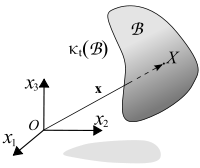
\includegraphics[scale=0.75]{Continuum_body}\\

\section {Non-local mechanics}
This theory assumes that the stress state at a reference point $\mathbf{x}$ in
the body is regarded to be dependent not only on the strain state at
$\mathbf{x}$ but also on the strain states at all other points $x$ of the body. The
most general form of the constitutive relation in the nonlocal
elasticity type representation involves an integral over the entire
region of interest. The integral contains a nonlocal kernel function,
which describes the relative influences of the strains at various
locations on the stress at a given location. The constitutive
equations of linear, homogeneous, isotropic, nonlocal elastic solid
with zero body forces are given by\\
\begin{equation}
\sigma_{ij,j}=0
\end{equation}
\begin{equation}
\sigma_{ij}(\mathbf{x})=\int_V \alpha(|\mathbf{x-x'}|,\xi)C_{ijkl}\epsilon_{kl}(\mathbf{x'})dV(\mathbf{x'}),\qquad \forall x \in V \label{eqNL}
\end{equation}
\begin{equation}
\epsilon_{ij}=\frac{1}{2}(u_{i,j}+u_{j,i})
\end{equation}
where $C_{ijkl}$ is the elastic modulus tensor of classical isotropic
elasticity, $\sigma_{ij}$ and $\epsilon_{ij}$ are stress and strain tensors, respectively,
and $u_i$ is the displacement vector. $\alpha = \alpha(|\mathbf{x-x'}|,\xi)$ is the nonlocal
modulus or attenuation function incorporating the nonlocal effects
into the constitutive equations. This nonlocal modulus is found by
matching the curves of plane waves with those due to atomic lattice
dynamics. Various different forms of $\alpha(|\mathbf{x-x'}|)$ have been reported in \cite{eringen1976nonlocal} .$|\mathbf{x-x'}|$ is the Euclidean distance, and $\xi = e_0 a/l$\cite{peddieson2003application} where a is an internal characteristic length, e.g., length of C–C bond
(0.142 nm) in CNT, granular distance etc., and $l$ is an external
characteristic length e.g., wavelength ($\lambda$) , crack length, size of the
sample etc. $e_0$ is a nonlocal scaling parameter, which has been
assumed as a constant appropriate to each material in published
literature and V is the region occupied by the body. Choice of the
value of parameter $e_0a$  (in dimension of length) is crucial to ensure
the validity of nonlocal models. This parameter was determined by
matching the dispersion curves based on the atomic models\cite{eringen1983differential}. For
a specific material, the corresponding nonlocal parameter can be
estimated by fitting the results of atomic lattice dynamics or
experiment.

The generally used kernel function $\alpha(|\mathbf{x-x'}|,\xi)$ used in \ref{eqNL} is given in \cite{eringen1972linear}:\\
\begin{equation}
\alpha(|\mathbf{x-x'}|,\xi) = \dfrac{1}{2 \pi \xi^2 l^2} K_0\left(\frac{\bf{x.x}}{\xi l}\right)
\end{equation}
where $K_0$ is is the modified Bessel function.
For two-dimensional nonlocal elasticity, there exists a differential form for the stress–strain relation (from \eqref{eqNL})\cite{eringen1972linear,eringen1976nonlocal,eringen1983differential,eringen1972nonlocal}\\
\begin{equation}
\left(1-\xi^2 l^2 \nabla^2\right)\sigma_{ij} = C_{ikjl}\epsilon_{kl} \label{NLconsteqn}
\end{equation}
where the operator $\nabla^2$ is the Laplacian operator. Notice that in the
nonlocal elasticity, the effect of small-length scale is considered by
incorporating the internal parameter length into the constitutive
equation. One may also see that when the internal characteristic
length $a$ is neglected, i.e., the particles of a medium are considered
to be continuously distributed, then $\xi =0$ and \eqref{NLconsteqn} reduces to the
constitutive equation of classical elasticity. When the internal
characteristic length is negligible compared to external characteristic length, $\xi$ approaches zero and hence nonlocal elasticity theory reduces to classical elasticity theory. While the internal characteristic length is reasonably close to external characteristic length, $\xi$ approaches to unity and thus the nonlocal elasticity
theory reduces to atomic lattice dynamics. For nanostructures, the
internal and external lengths are of the same order, and one has to
use the nonlocal theory for analysis.
\subsection{Discussion on nonlocal small scale coefficient}
The identification of the small scaling parameter $e_0$ in the
nonlocal theory has not been fully understood. Wang and Hu \cite{wang2005flexural},
who adopted the second order strain gradient constitutive relation,
proposed $e_0 = 0.288$ for the flexural wave propagation study in a
single-walled carbon nanotube (SWCNT) through the use of
nonlocal Timoshenko beam model and molecular dynamic simulations (MDSs).Eringen \cite{eringen1983differential} himself proposed $e_0$ as 0.39 based on the
matching of the dispersion curves via nonlocal theory for plane wave and Born-K\'arm\'an model of lattice dynamics at the end of
the Brillouin zone, $k \times a = \pi$ where $a$ is the distance between atoms
and $k$ is the wave number in the phonon analysis. On the other
hand, Eringen \cite{eringen1972linear}proposed $e_0 =0.31$ in his study on the comparison of the Rayleigh surface wave via nonlocal continuum mechanics
and lattice dynamics. Zhang et al.\cite{zhang2005free} estimated $e_0=0.82$ from the buckling analysis of SWCNT via Donnell shell theory and molecular
mechanics simulations. Zhang et al.\cite{zhang2006atomistic} performed analysis of
elastic interactions between Stone–Wales and divacancy defects on
carbon graphene sheet. They concluded that the displacement field
around defects obtained from the nonlocal continuum model and
MDSs can match very well if $e_0$ is chosen to be $8.79$  The varied
values of $e_0$ prompted Wang \cite{wang2005wave} to state that the adopted value of
the scaling parameter $e_0$ depends on the crystal structure in lattice
dynamics and the nature of physics under investigation. He also
estimated that the scale coefficient $e_0 < 2.0$ nm for a SWCNT if the
measured wave propagation frequency value is assessed to be
greater than 10 THz. Although $e_0$ is a key parameter in the nonlocal
elasticity theory, there is hitherto no rigorous study being made on
estimating the scaling parameter $e_0$ for various physical problems.
Hu et al.\cite{hu2008nonlocal} estimated the value of parameter $e_0$ is estimated
based on the MD result to predict the dispersion of transverse wave
in CNTs through using the nonlocal shell models. The results of
their study indicate that the nonlocal elastic cylindrical shell model
is able to offer a better prediction for transverse and torsional wave
dispersion in CNTs than the local elastic shell model when the
wavenumber is large enough. They also show that the nonlocal
shell models are required when the wavelengths are approximately
less than $2.36 \times 10^{-9} \text{ and } 0.95 \times  10^{-9}$m for transverse wave in armchair (15,15) SWCNT and torsional wave in armchair (10,10)
SWCNT, respectively. Following Wang \cite{wang2005wave}, the nonlocal parameter $e_0a$ should be less than 2.0 nm, so that here in the simulation procedure we choose
$e_0a = 0.0, 0.5\text{ and }1.0 $ nm, respectively.

